\chapter{Evaluation}

%EL schemas enable consistent, structured, and interpretable inferences about novel text, by matching pieces of the text to pieces of the schema, replacing schema variables with entities from the story, and treating other formulas in the schema that use those newly-filled variables as inferences. Here, we describe an assessment of the generality and relevance of the schema formulas learned by NESL.
%In addition to inferences, we would like to evaluate whether the schemas we obtain are both \textit{topically cohesive}, i.e., focused descriptions of one kind of situation; and \textit{interesting}, i.e., capable of generating useful and novel inferences about situations, rather than obvious or redundant ones.
This chapter describes experiments performed to assess the quality of schemas learned by NESL, and of inferences generated by learned schemas on unseen stories.
One way of evaluating acquired script-like knowledge is the \textit{narrative cloze} task, introduced by \citet{chambers2008unsupervised}, in which one event in a sequence is masked, and acquired knowledge is used to predict its identity given the rest of the sequence.
The narrative cloze task has been widely adopted as a standard evaluation for script-like knowledge acquisition \citep{jans-etal-2012-skip,rudinger-etal-2015-learning,pichotta2016learning,lee-goldwasser-2019-multi}.
However, \citet{rudinger-etal-2015-learning} note that the format of the narrative cloze task essentially mirrors that of a language model objective function, in which a missing token is predicted given a preceding sequence (in the autoregressive objective) or surrounding sequences (in the masked objective).
They argue that either discriminative language models are sufficient for the acquisition of script knowledge, or the narrative cloze task is insufficient for its evaluation.
\citet{chambers-2017-behind} defends the event cloze task by pointing out that many of its implementations, in automatically generating their evaluation sets, tested for non-representative distributions of events favoring high-frequency ones.
They argue for manual construction of narrative cloze tests by human annotators, with an emphasis on the inclusion of \textit{core} script events.

While NESL uses a generative language model to produce stories as an initial source for schema knowledge, the knowledge encoded in the final schemas is not drawn from the same distribution as the one producing the stories; stories often elide basic, but important, information about goals, preconditions, postconditions, and general semantic role types, which we introduce via protoschema identification. Furthermore, generative models of stories may call for the introduction of surprising events or facts in accordance with larger-scale \textit{narrative} schemas---this to the semantic detriment of the more basic, unsurprising schemas we'd like to extract from stories. Because of these factors contributing to the potentially highly disjoint event spaces of individual stories and learned schemas, we believe that a narrative cloze task is insufficient to test the quality and utility of the inferences generated by NESL-learned schemas, and employ human evaluation of learned schemas and their inferences. The remainder of this chapter describes the evaluation of schema steps and goals given the schema topic (Section~\ref{sec:schema_eval}), and the evaluation of concrete inferences, drawn using learned schemas, about unseen stories (Section~\ref{sec:inf_eval}).

\section{Schema Evaluation}
\label{sec:schema_eval}

\begin{figure}
    \centering
    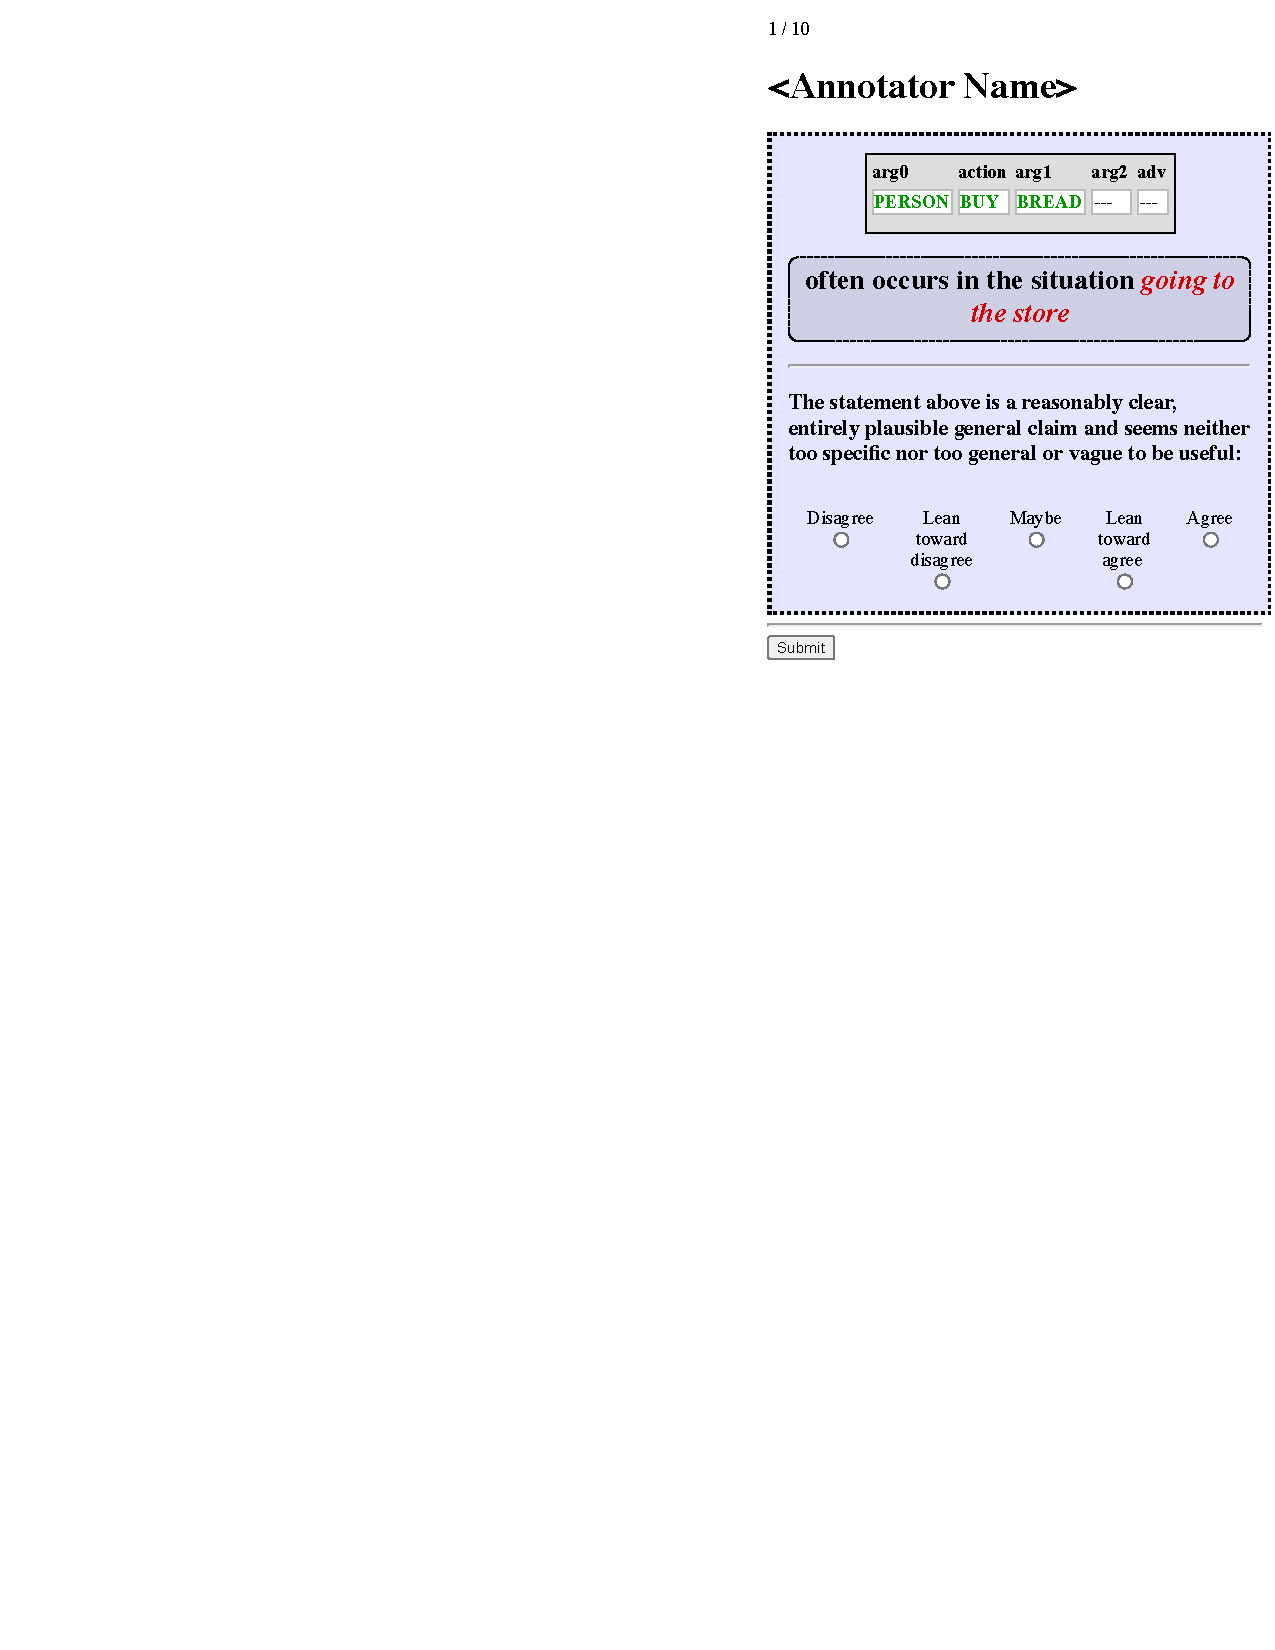
\includegraphics[width=0.5\textwidth]{CH4_learning/evaleg3.pdf}
    \caption{An example of a form presented to a schema quality evaluator for a \textit{step} formula.}
    \label{fig:step_eval_eg}
\end{figure}

\begin{figure}
    \centering
    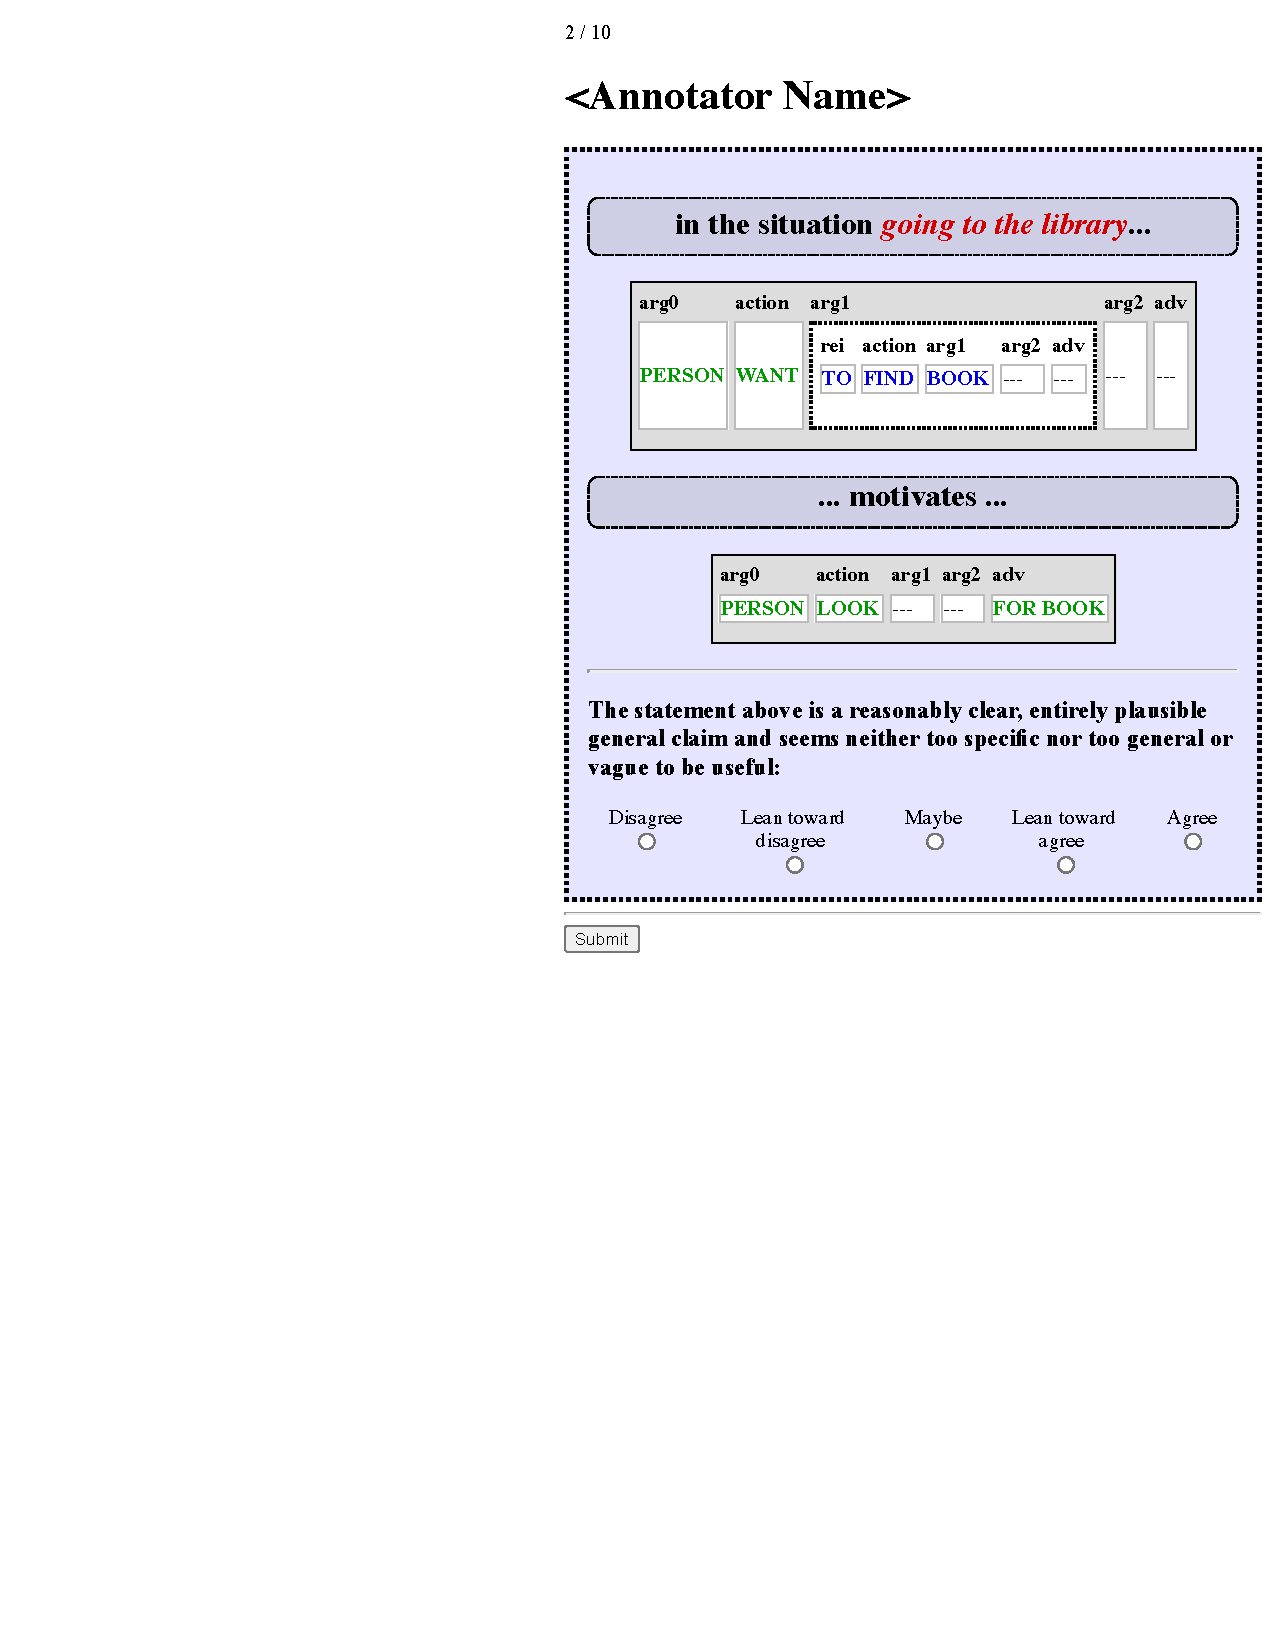
\includegraphics[width=0.5\textwidth]{CH4_learning/evaleg4.pdf}
    \caption{An example of a form presented to a schema quality evaluator for a \textit{goal} formula.}
    \label{fig:goal_eval_eg}
\end{figure}

\section{Inference Evaluation}
\label{sec:inf_eval}

\begin{figure}
    \centering
    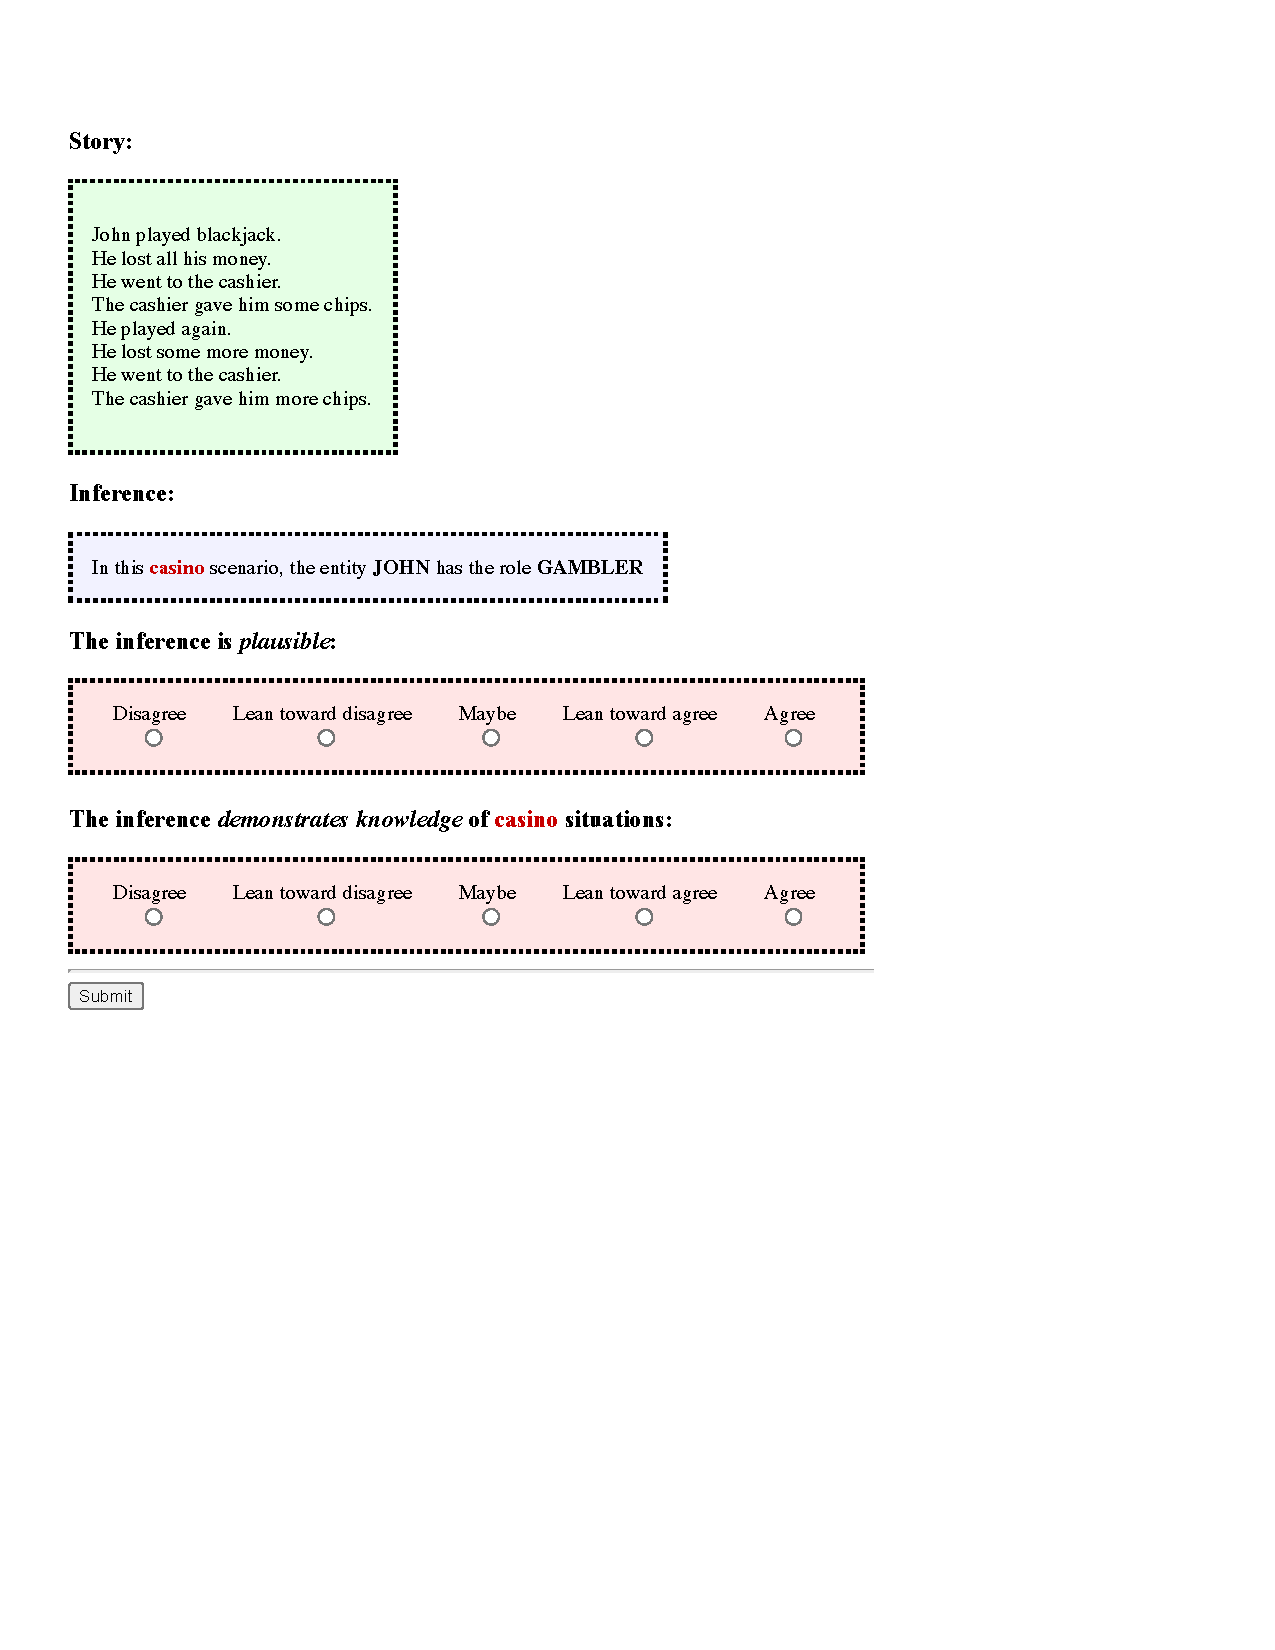
\includegraphics[width=\textwidth]{CH5_eval/role_inf.pdf}
    \caption{An example of a form presented to a schema quality evaluator for a \textit{goal} formula.}
    \label{fig:role_inf_eval}
\end{figure}

\begin{figure}
    \centering
    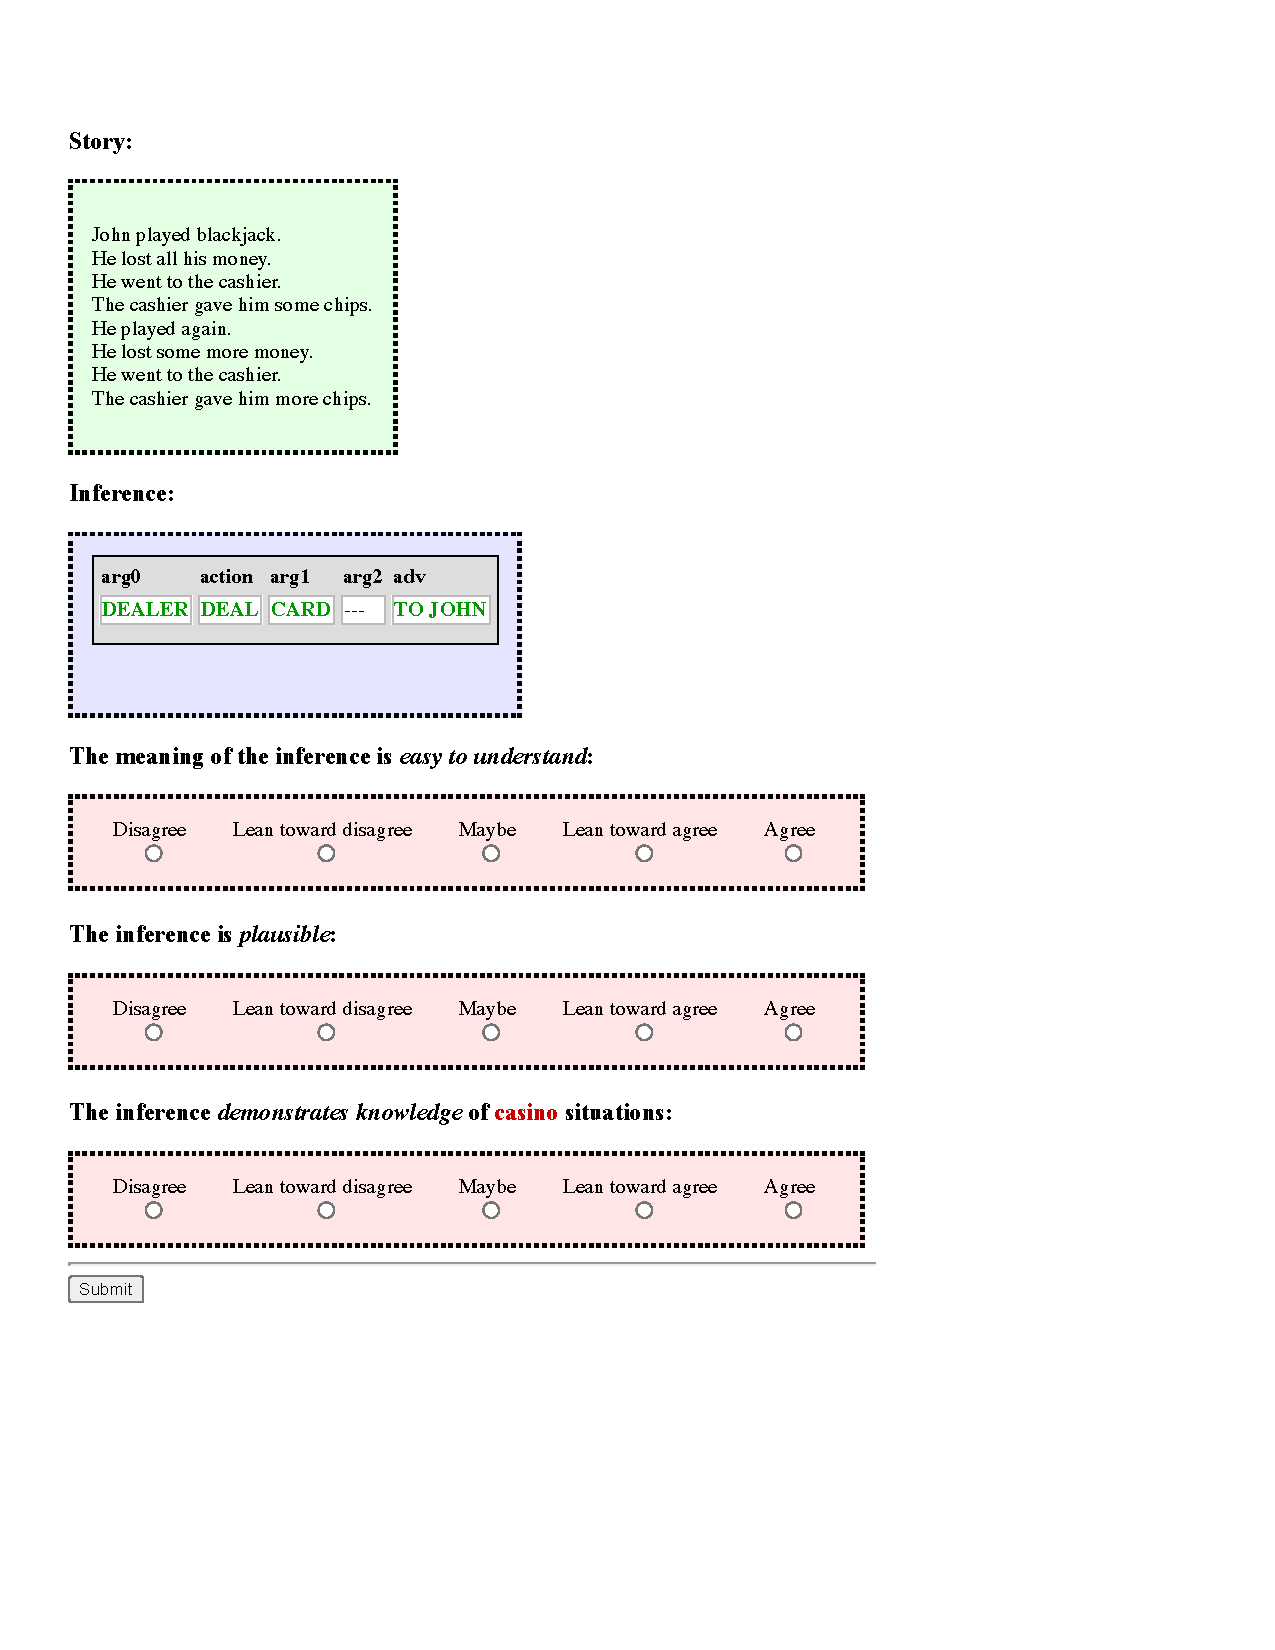
\includegraphics[width=0.75\textwidth]{CH5_eval/step_inf.pdf}
    \caption{An example of a form presented to a schema quality evaluator for a \textit{goal} formula.}
    \label{fig:step_inf_eval}
\end{figure}